\documentclass[12pt]{article}
\usepackage[utf8]{inputenc}
\usepackage[font={small},labelfont=bf]{caption}
\usepackage{lmodern}
\usepackage[left=3cm, right=3cm, top=3cm, bottom = 2cm ]{geometry}
\usepackage[utf8]{inputenc}
\usepackage[T1]{fontenc}
\usepackage{microtype}
\usepackage[dvips]{graphicx}
\usepackage{xcolor}
\usepackage{times}
\usepackage{gensymb}
\usepackage{cite}
\usepackage{amsmath, amssymb, amsthm}
\usepackage{siunitx}
\usepackage{underscore}
\usepackage{url}
\usepackage{float}
\usepackage{booktabs}
\usepackage{float}
\usepackage[parfill]{parskip}
%\usepackage{cite} % takes care of citations
\usepackage[final]{hyperref} % adds hyper links inside the generated pdf file
\usepackage{wrapfig}
\hypersetup{
	colorlinks=true,       % false: boxed links; true: colored links
	linkcolor=blue,        % color of internal links
	citecolor=blue,        % color of links to bibliography
	filecolor=magenta,     % color of file links
	urlcolor=blue         
}
%\usepackage{minted}
%\large
%\title{TITLE}

\begin{document}
\begin{titlepage}
	\begin{center}
    \line(1,0){300}\\
    [0.65cm]
	\huge{\bfseries Probabilistic BLAST: a probabilistic sequence alignment algorithm using a bidirectional hidden Markov Model}\\
	\line(1,0){300}\\
	\textsc{\Large Tim Liu, Yifan Zhao}\\
	\textsc{\LARGE December 11, 2019}\\
	[5.5cm]     
	\end{center}

\end{titlepage}

\tableofcontents


\clearpage










\label{Introduction}
\section{Introduction}
Sequence alignment algorithms are widely used in bioinformatics to search for the similarity between input sequences of DNA, RNA or protein. There are two main kinds of sequence alignment algorithms: global alignments and local alignments. Global alignment rearranges the entire length of the input sequences. On the other hand, local alignment looks for the similar regions between short query and long database. A good sequence alignment algorithm is able to produce high-quality sequence alignments efficiently. However, it is hard to build an algorithm that is fast and guaranteed for optimal outcomes \cite{polyanovsky2011}. 

In certain situations, scientists may not know exactly the genome of a species, but instead there exists some uncertainty about the identity of nucleotides at a given position. Since the genome for a species is not clear to form a linear sequence, a probabilistic matrix is built to represent the uncertainty of the nucleotides on each position of the genome. With probabilistic setting, the genome cannot be aligned with an input query with general linear sequence alignment algorithms. To this end, we aim to develop alignment algorithms that can fulfill the need of probabilistic sequence alignment with high efficiency and accuracy. 

%%%%%%%%%%%%%BACKGROUND START%%%%%%%%%%%%%

\label{Background}
\section{Background}
In this project, the goal is to find alignments between a short linear sequence and a long probabilistic genome. HMMER is a sequence analysis tool used for searching homologous sequences and making alignments \cite{eddy2009}. It includes probabilistic models called profile hidden Markov models (profile HMM). HMMER has higher accuracy than Basic Local Alignment Searching Tool (BLAST), a widely used algorithm for sequence comparison. However, the slower speed of HMMER limits its performance and application. Therefore, for this project, we chose to approach BLAST-based algorithm to find the balance between running time and accuracy. Borrowing ideas from the general BLAST algorithm, we created a novel probabilistic sequence alignment algorithm, probabilistic BLAST (“pBLAST”).

%%%%%%%%%%%%%BACKGROUND END%%%%%%%%%%%%%

%%%%%%%%%%%%%MATERIALS START%%%%%%%%%%%%%

\label{Materials}
\section{Materials}
All the tests and evaluation are run on a macOS 10.14 system with a i7 core processor and 16GB RAM. All of the scripts written for this study can be found in our  \href{https://github.com/yifnzhao/probabilistic-sequence-alignment}{GitHub Repository}.

\subsection{Probabilistic genome dataset}
In this study, a probabilistic genome dataset from a portion of chr22 of a predicted Boreoutherian ancestor sequence is used for testing and evaluation. The raw data consists of the predicted sequence with corresponding confidence (from 0 to 1), p,  at each position. For each position, the nucleotides different than the one that appears in the predicted sequence, share the same probability, $\frac{1}{3}(1-p)$.

\label{queryGeneration}
\subsection{Probabilistic genome query generation}
In order to test the algorithm, a query generator is built to create query sequences with different lengths (25, 50, 100, 200, or a random integer between 6 and 200) and starting positions. The query generator also uses a parameter, weight, to define the probability of a position in the generated query having the most probably nucleotide from the input database. For each position in the query sequence from starting position until the desired length is reached, the query generator randomly generates a number, \textbf{p}, between 0 and 1. If \textbf{p} is smaller or equal to the weight, the nucleotide with the highest occurrence probability would be chosen. If \textbf{p} is greater than the weight, query generator will randomly choose one of the other three nucleotides. The true probability for the queries is also recorded for evaluation purposes in later steps. 


%%%%%%%%%%%%%MATERIALS END%%%%%%%%%%%%%




%%%%%%%%%%%%%METHODS START%%%%%%%%%%%%%
\label{Methods}
\section{Methods}

\subsection{General BLAST algorithm}
The general BLAST is used to search for a given query sequence in a genome database to find out any local similarity between them. It takes sequences and weight matrix as inputs and then outputs the alignments for the input sequence and a table with scoring related data when performing on NCBI. BLAST uses a heuristic method to find provably  good alignments between the input query and the database according to a scoring scheme, but the results are not guaranteed to be optimal. Because its strategy is to find as many matches as possible, it is less sensitive than alignment methods that guarantee optimal alignment such as Needleman-Wunsch algorithm \cite{needleman1970}. 

The general BLAST algorithm requires a sequence database to compare with input queries. However, probabilistic sequences are not linear  sequences which can be directly used for comparison. In a probabilistic genome database, the probabilities of  each nucleotide occurring at a specified position are stored in a matrix, i.e.,  there is no actual nucleotide assigned in any position along the reference  sequence. Therefore, the general BLAST algorithm needs to be modified to accomodate the need of  sequence alignment to probabilistic genome database. Our approach, termed probabilistic BLAST (“pBLAST”) , consists of three main steps: seeding, extension, and evaluation.

\subsection{Seeding}
Seeding is the initial step for pBLAST to locate all the similarities between a query and the database. The query is divided into a list including every possible w-length word (also called a seed) along the query, where w is a user-defined parameter in the pBLAST algorithm. Then, for each seed in the list, pBLAST scans through the database to find regions of perfect match and store them for further investigation. There are two different methods of seeding with probabilistic settings approached in this project.

The first approach, seedS, concatenates all of the most probable nucleotides, i.e., the nucleotide with the highest probability at each position in the matrix, into one string (hereafter referred to as the “highest probability string”).  Next, pBLAST scans through the highest probability string to find all of the starting positions of perfect match regions for every seed in the list and stores them in a seeding position list.

In our second approach, seedM, pBLAST directly  scans the probability matrix. For every seed, pBLAST aligns it through the matrix and find the position with the highest probability, and then stores both the position and the probability. To qualify what a high probability seed is, two schemes can be applied: by specifying a fixed number of seeding positions to look for, or by setting a minimum probability threshold for a seed alignment. By applying either of the schemes above, the seeding position list will be narrowed down and ready for extension phases.

\subsection{Extension}
Once pBLAST finds the high quality seeds from the seeding method and their corresponding start positions of the selected seeds , the next step is to extend these hits to collect high-scoring segment pairs (HSPs). Similar to the general BLAST, pBLAST has two phases of extension: an ungapped extension phase followed by a gapped extension phase.

In the ungapped extension phase, pBLAST converts the seed hits into ungapped alignments along the database and then search for HSPs. In a standard BLAST ungapped extension, the total score of the alignment oscillates and can increase due to the fact that the score is calculated using a substitution matrix. As a result, the alignment score is expected to increase when a high-scoring pair is aligned while extending a hit.  The BLAST version ungapped phase ends when the score is almost strictly decreasing, and then start and end positions at which the hit has a peak score is reported as the start and end positions of the desired HSP. In pBLAST, however the total score of the alignment is computed as the product of the nucleotide probability at each position of the potential HSP at the current step. For probabilistic sequences, it is impossible to tell whether an alignment is getting “better” based on the probability score alone, because the probability score  always decreased as the hit becomes longer. In order to find the HSPs for probabilistic database, a three-state HMM is built and Viterbi algorithm is used to find its maximum likelihood path, i.e. an HSP. 
	
    \begin{wrapfigure}{r}{0.5\textwidth}
        \centering
		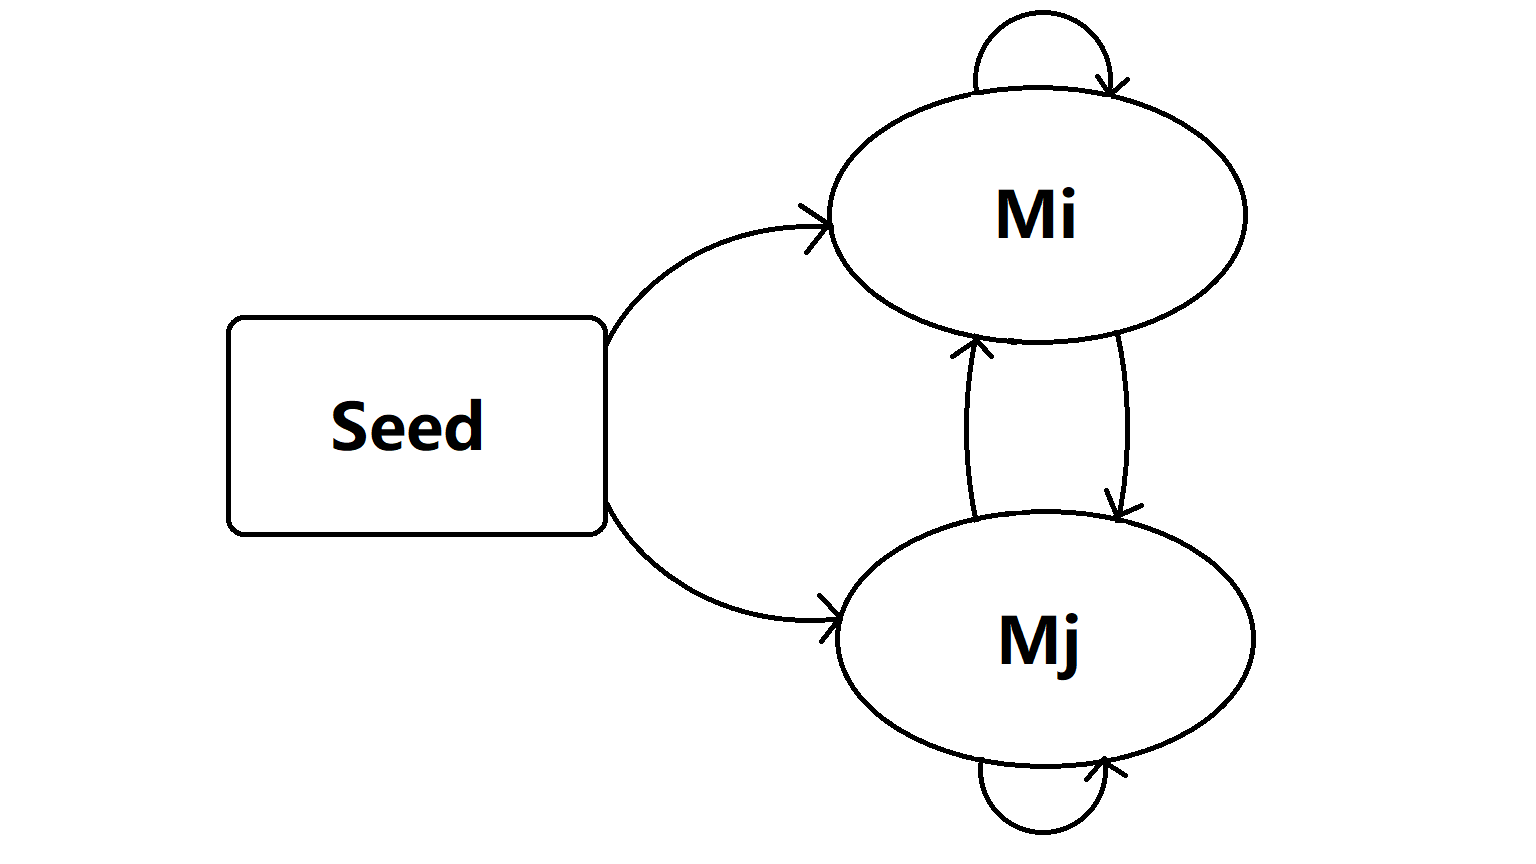
\includegraphics[width=0.5\textwidth,trim={0.5cm 0.5cm 0.5cm 0cm},clip]{fig3} % trim = {left lower right upper}
		\caption{\textbf{HMM graph of ungapped extension.}}
		\label{fig:ugappedHMMGraph}
	\end{wrapfigure}

An extension can occur at either ends of the seed. The Mi and Mj states represent the extensions on the left and right ends, respectively. In our naive implementation, the transition probabilities of staying on one end and transitioning to the other end have the same value, 0.5. In practice, the transition matrices could be modified to reflect the actual frequency statistics. The emission probability matrices inside Mi and Mj are also the same and based on the given probabilistic sequences. Ungapped extension concretizes the seed list according to the probability scores of the HSPs selected by the Viterbi algorithm.

After ungapped extension phase, the next step is to realign the seeds to the database with gapped alignment, and then select a portion of the high-scoring alignments. Directly starting the gapped extension from hsp is also a solution, but it will leaves a long gap-free region in the middle of its outcome alignment. Because it is unrealistic in biosequence alignment to have a long gap-free middle region, then the gapped extension is designed to start with the seeds again. When gapping the sequences, gaps of three or multiples of three are more preferred than the other gaps, because amino acids are coded by three nucleotides and gaps of three would not induce deleterious frameshift program on the sequence. Unlike the ungapped extension, the HMM model for gapped phase is more complicated. Assume the extension only happens on one end of the seed, a four-state HMM is created.
	
    \begin{figure}[!htb]
            \centering
		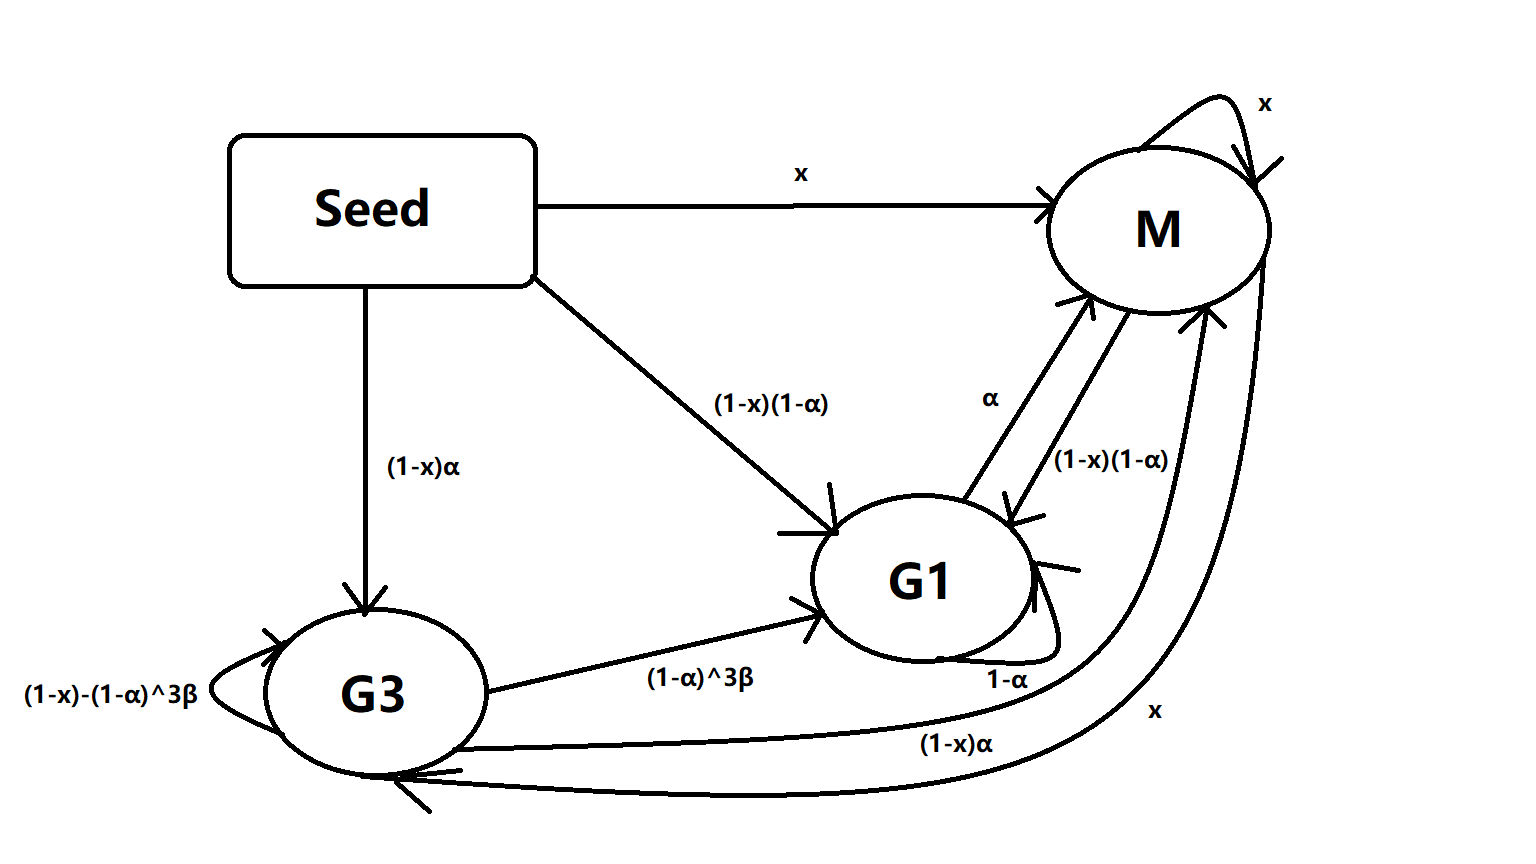
\includegraphics[width=0.65\textwidth,trim={0.5cm 1cm 2cm 0.5cm},clip]{fig4} % trim = {left lower right upper}
		\caption{\textbf{HMM graph of half gapped extension.}}
		\label{fig:halfGappedHMMGraph}
	\end{figure}

There are three parameters in the HMM: \textbf{$\alpha$} is the probability of gaps of three; \textbf{$\beta$} is the number of G3 gone through; \textbf{x} is the transition probability to M. G3 is the state for gaps of three and G1 is for other gaps. The emission probability of M state is based on the given probabilistic database and of G1 and G2 are all 1 because gap states have only gaps as their outcomes.
    
    \begin{figure}[!htb]
        \centering
		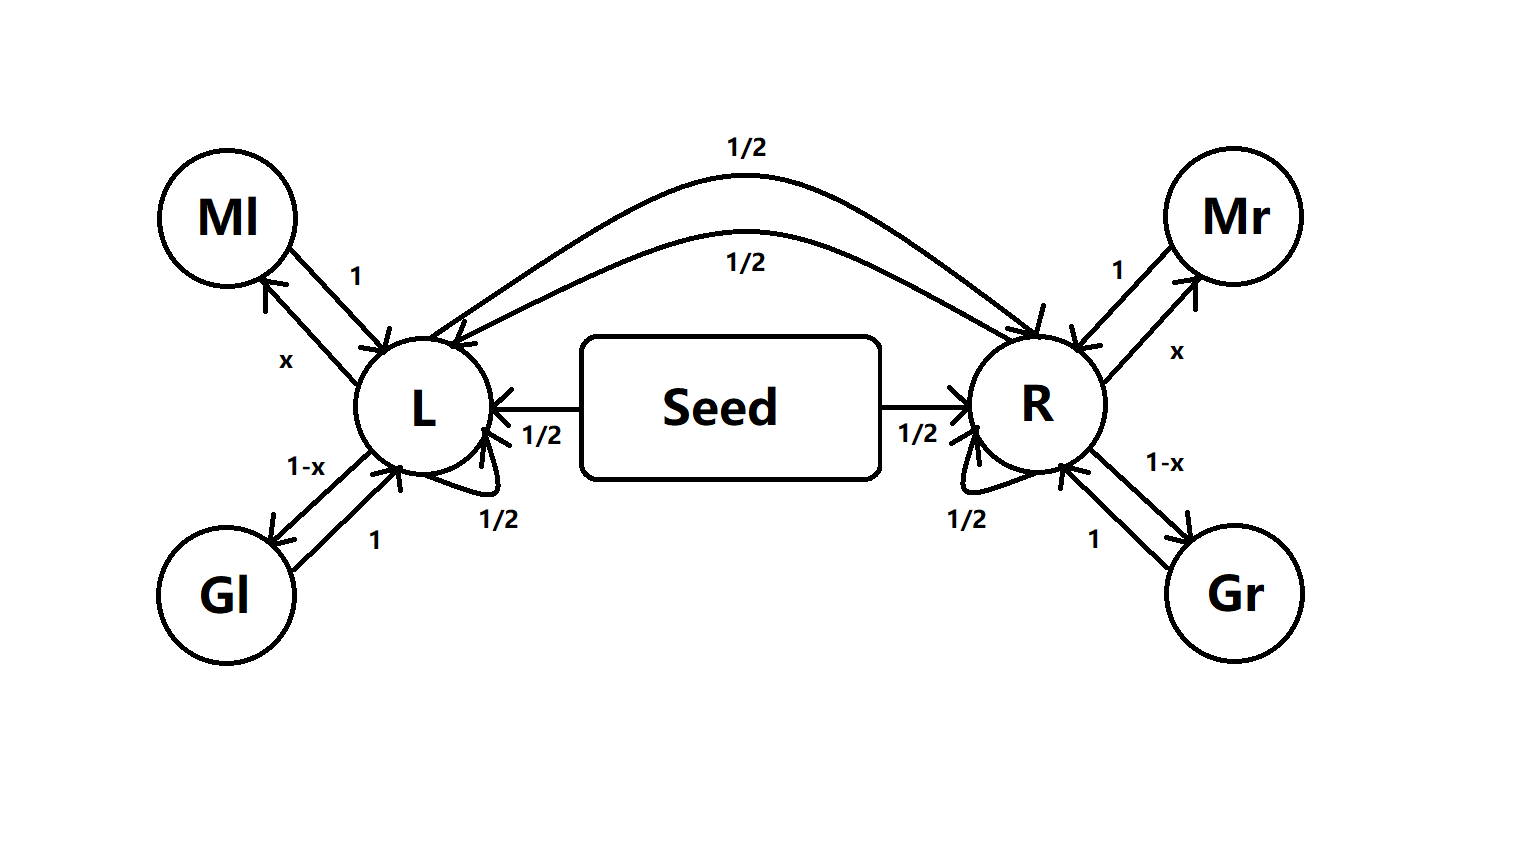
\includegraphics[width=0.7\textwidth,trim={0.5cm 5cm 3cm 0.5cm},clip]{fig5} % trim = {left lower right upper}
		\caption{\textbf{HMM graph of gapped extension.}}
		\label{fig:gappedHMMGraph}
	\end{figure}
Like the ungapped phase, gapped alignment takes place on both ends of the seed, so the HMM should have two sets of match and gap states: Mi, G1i, G3i, Mj, G1j, and G3j. However, the complete HMM is not a simple duplicate of the partial HMM above, because there must be some restrictions for transition between two ends to make the model valid. For example, when transiting from left end to right end, if the last visited right-end state is G1r, then the probability for transition to G3r should be zero, because G1r cannot transit to G3r in general. Therefore, the transition probability across the ends should depends on the last visited state on the destination end. The HMM becomes too complicated to model after considering these restrictions. As a solution, merge the gap states together and convert the transition probability of them to emission probability inside the new gap state. Then, add L and R states represent extension on left or right end of the seed.


%%%%%%%%%%%%%METHODS END%%%%%%%%%%%%%
%\clearpage

%%%%%%%%%%%%%RESULTS START%%%%%%%%%%%%%
\label{Results}
\section{Results}

	\begin{figure}[!htb]
		\centering
		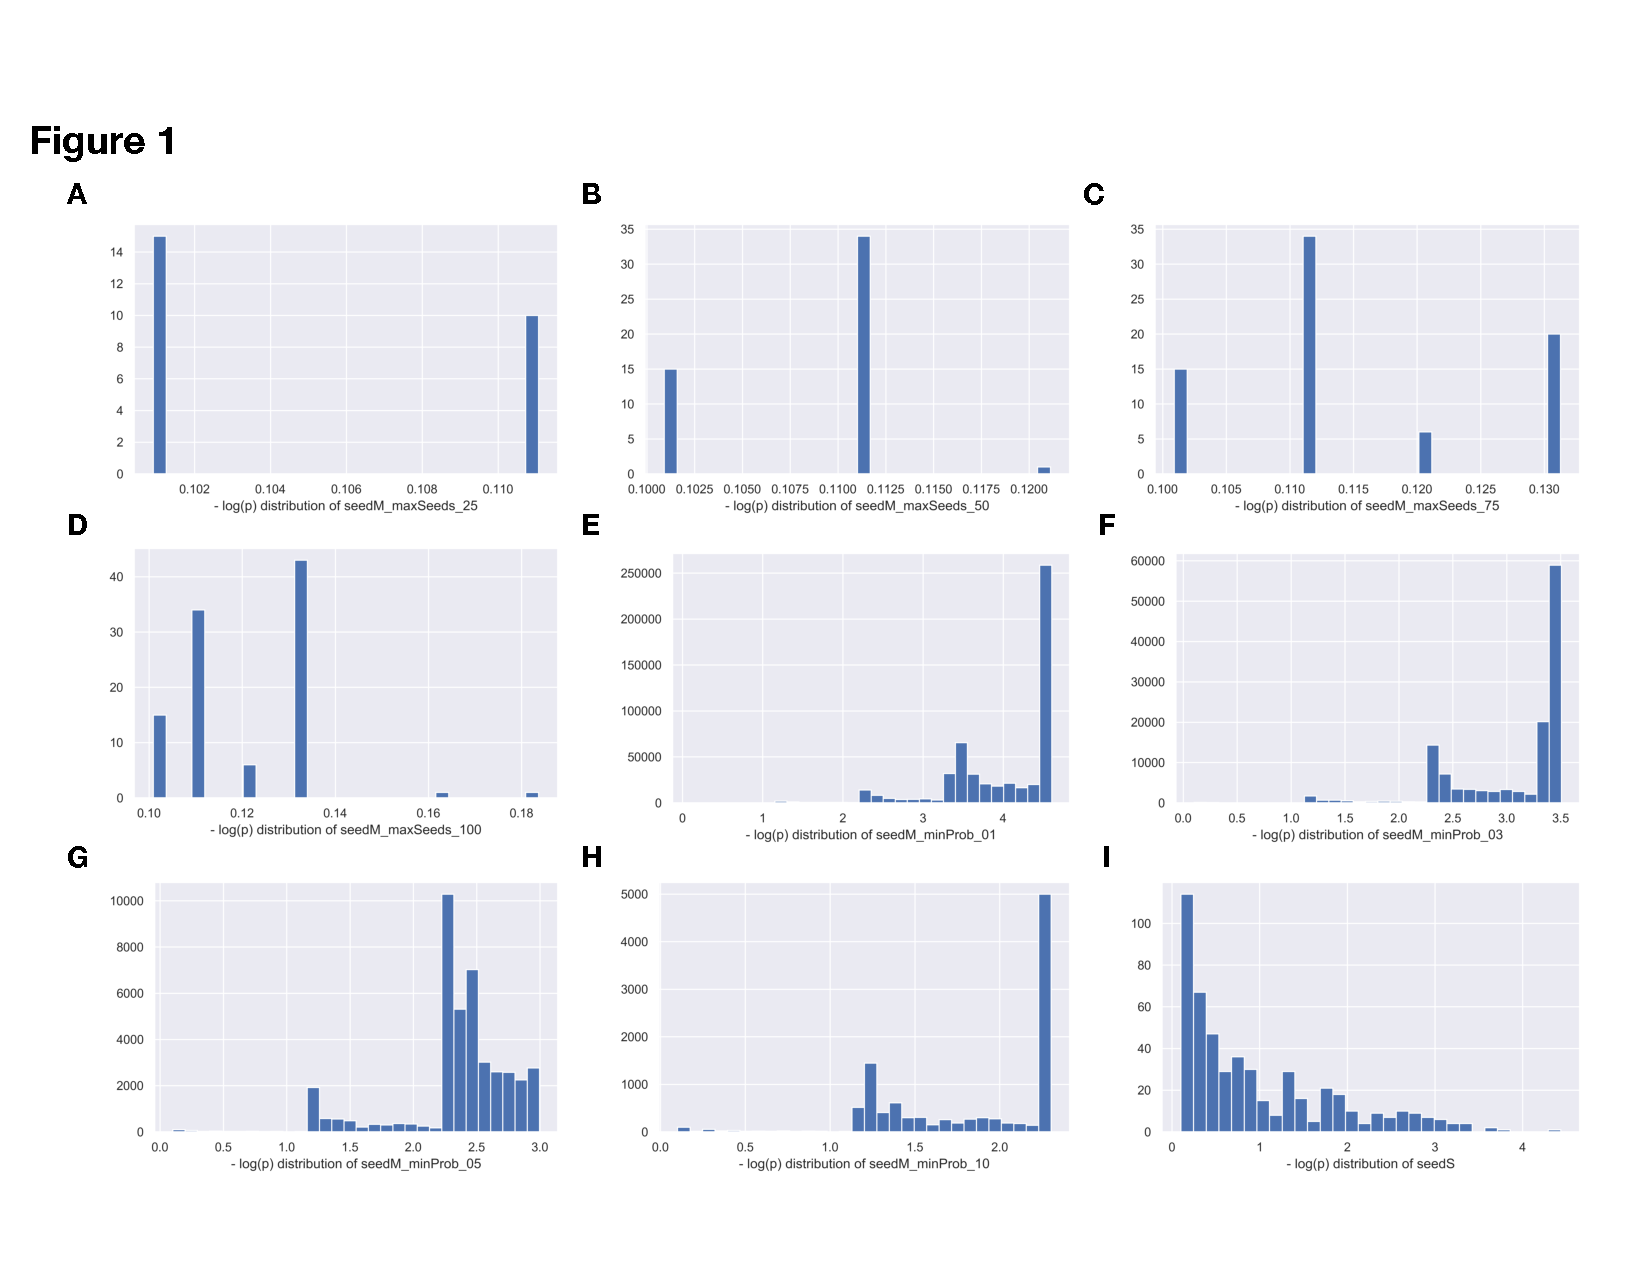
\includegraphics[width=1\textwidth,trim={0.5cm 1cm 0.7cm 3cm},clip]{fig1} % trim = {left lower right upper}
		\caption{\textbf{Representative probability distribution of 3 types of seeding methods.} \textbf{(A)-(D):} SeedM with fixed seed list size of 25, 50, 75, 100, respectively. \textbf{(E)-(H):} SeedM with fixed lowest probability threshold of 0.01, 0.03, 0.05, 0.10, respectively. \textbf{(I):} SeedS. The query sequence is generated by choosing a random start point with fixed length of 25 and weight of 1.0 (see Section \ref{queryGeneration} Probabilistic genome query generation).}
		\label{fig:seedDistribution}
	\end{figure}
	

We first tested the performance of different seeding methods, \textit{seedM} and \textit{seedS}. Using the same query sequence, \textit{seedS} is the most efficient, taking $10^{-3}$ as much time as \textit{seedM} methods and has relatively high probability score on average (Figure \ref{fig:seedDistribution}, Table \ref{fig:seedTable}). The high efficiency of \textit{seedS} was expected due to the fact that the \textit{seedS} method reads a linear sequence whereas the \textit{seedM} methods read a four dimensional matrix. Within the \textit{seedM} method category, we investigated whether \textit{seedM} with fixed maximum number of \textit{seedS} (thereafter referred to as “\textit{seedM-n}”) or \textit{seedM} with minimum probability threshold (thereafter referred to as “\textit{seedM-p}”) yields better \textit{seedS}. We observed that as the maximum seed number decreases from 100 to 25, both accuracy and efficiency of \textit{seedM-n} increases. The observed trend could be explained by the fact that the “\textit{argmin}” step in \textit{seedM-n} to find the lowest probability seed (to be replaced) in the existing list is the most time consuming step.  As the size of seed list increases, \textit{argmin} takes more time to find the seed with lowest probability. On the other hand, the efficiency and accuracy of \textit{seedM-p} methods do not significantly vary with the threshold. However, we observed that all of the \textit{seedM-p} are significantly slower and less accurate than the \textit{seedM-n} methods. It is also worth noting that, while \textit{seedS} is significantly faster than \textit{seedM-n}, \textit{seedS} generates about 1000 as many \textit{seedS} as \textit{seedM-n} with n equals to 25. We expect that the large seed list size would affect the performance of downstream alignment steps. 

Although we implemented the ungapped extension phase using the HMM model and the baseline cutoff method (see Section \ref{Results} Results) to reduce seed list size and find HSPs, it has not been possible to test its performance without complete alignment output from the gapped extension phase. We also observed that as the seed position moves towards the center of the query sequence with respect to nucleotide positions, viterbi computation becomes increasingly costly in terms of both space and time (Figure \ref{fig:unappedDistribution}). If we have access to more powerful computers and more time, there are several tests and evaluation that could potentially be performed (see Section \ref{Discussion} Discussion).

    \begin{figure}[!htb]
		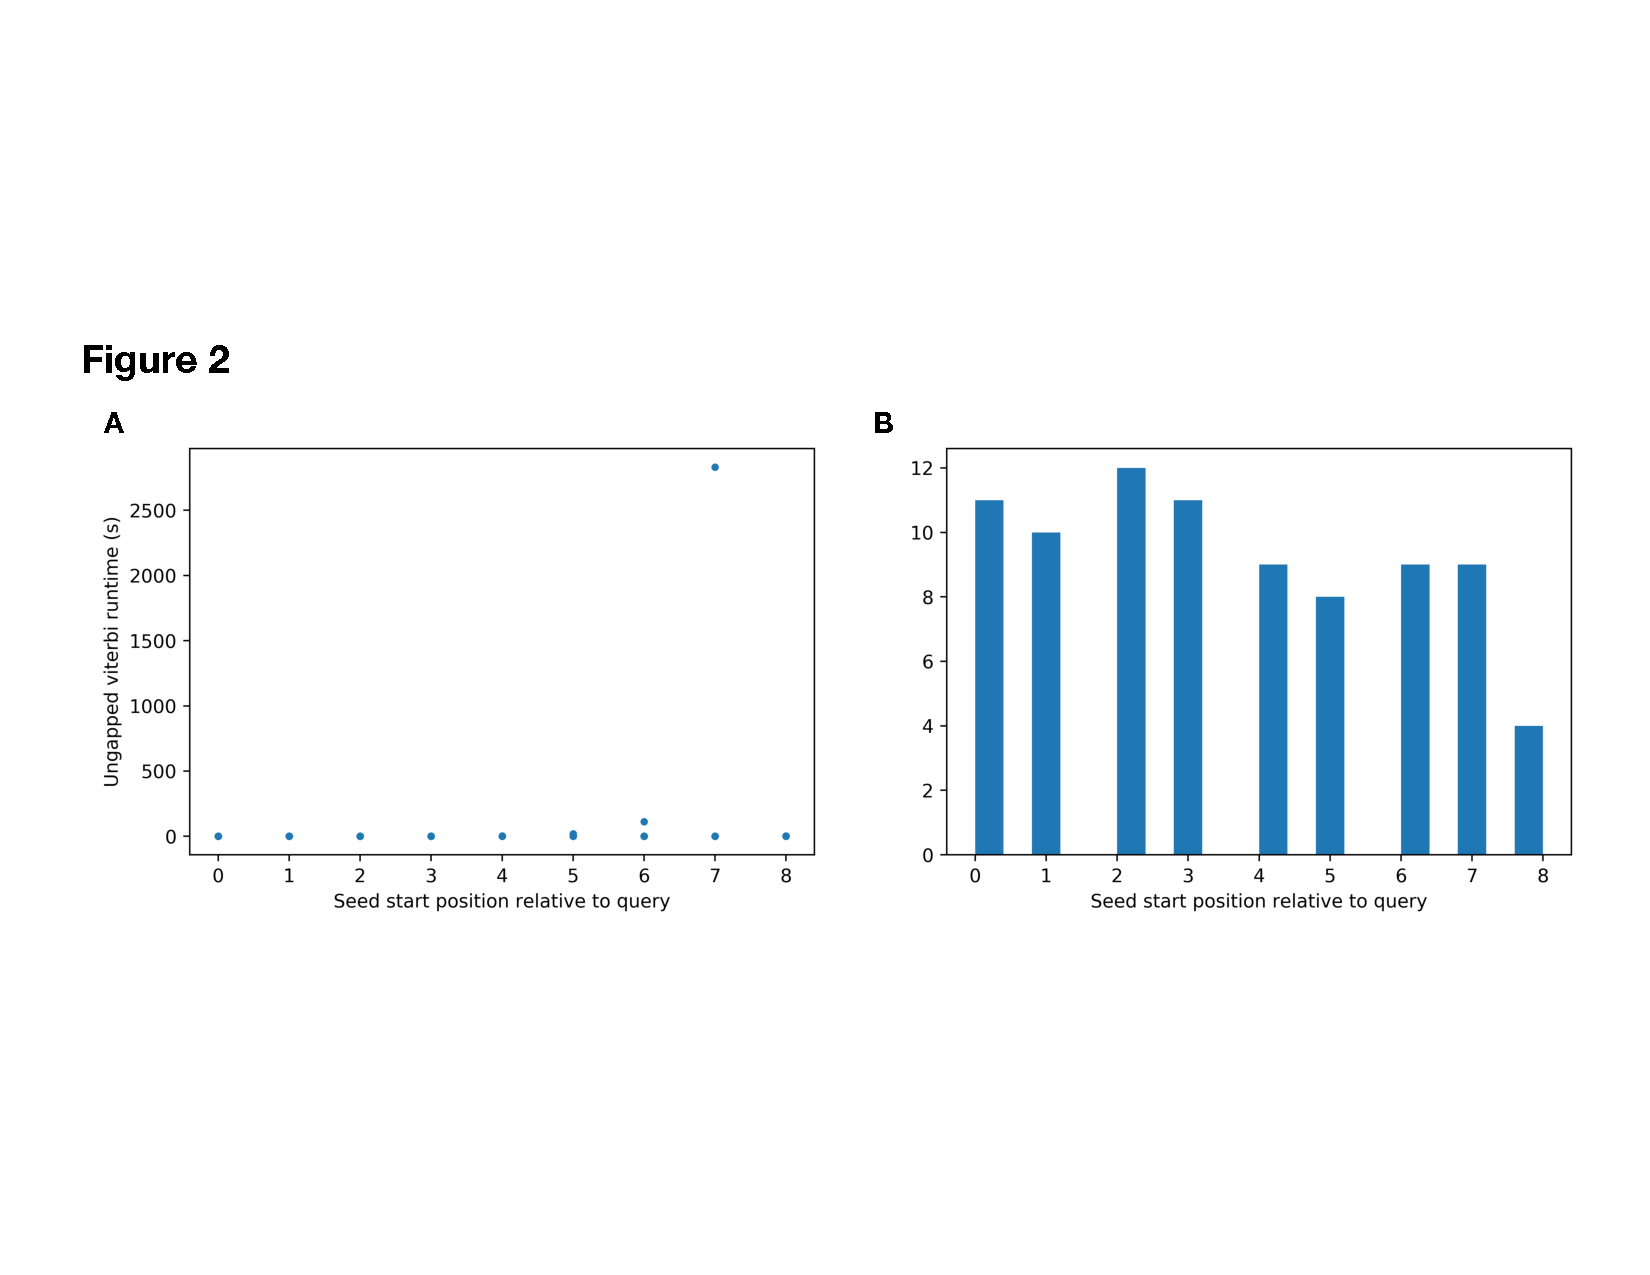
\includegraphics[width=1\textwidth,trim={0.5cm 6cm 0.5cm 6.8cm},clip]{fig2} % trim = {left lower right upper}
		\caption{\textbf{Ungapped viterbi computation becomes more costly as seed start position is further away from the query start (preliminary data).} \textbf{(A):} A representative scatter plot of ungapped viterbi runtime versus seed start positions. X-axis: seed start positions relative to the query sequence. Y-axis: runtime of ungapped viterbi function (in seconds). Note that the function was stopped prematurely as seed start position just reaches 8 due to time constraints. \textbf{(B):} Histogram of seed start position distributions for seeds that starts from position 0-8 that were used to generate the scatter plot on the left. Note that the bin of seed start position at 8 is an incomplete measurement of the actual number of the seeds that start at position 8 due to the premature stop as mentioned above.}
		
		
		
		\label{fig:unappedDistribution}
	\end{figure}	
	
	\begin{figure}[!htb]
		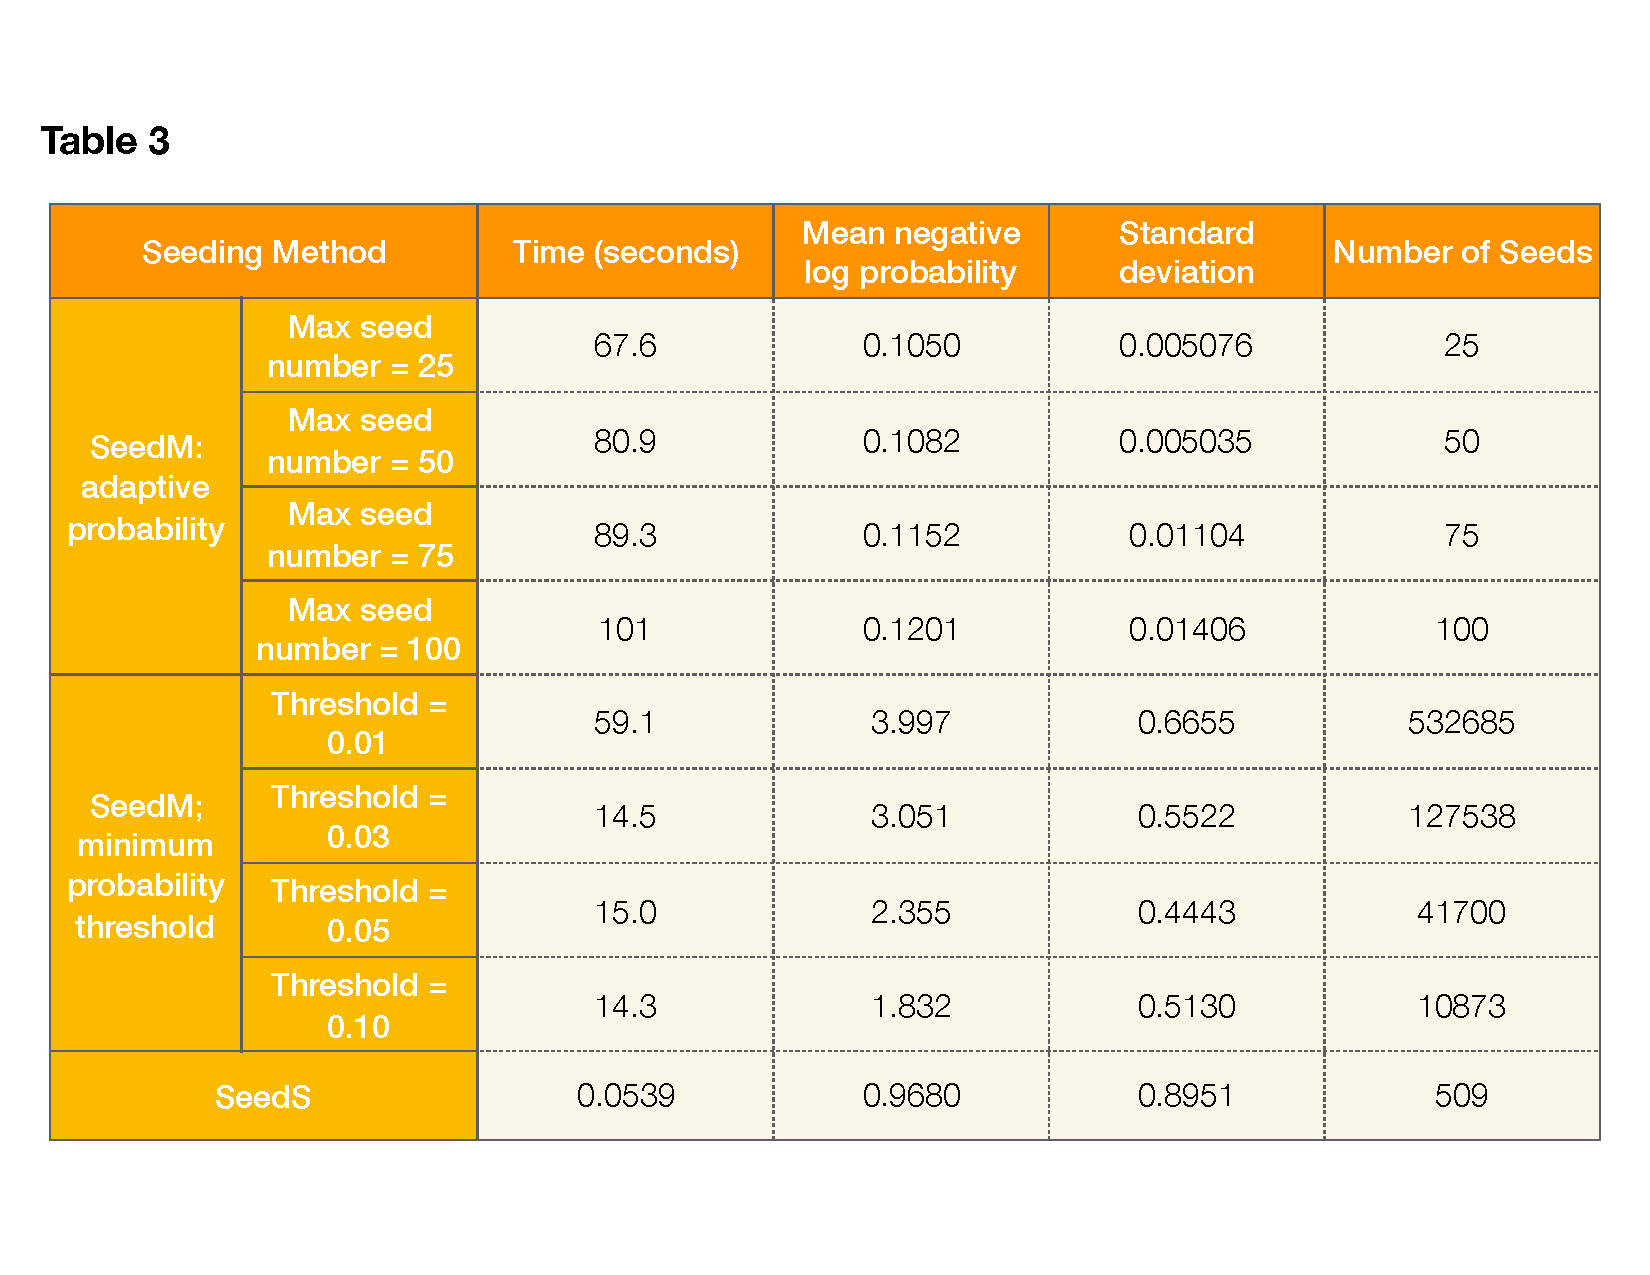
\includegraphics[width=1\textwidth,trim={0.5cm 2cm 0.5cm 5cm},clip]{tab3} % trim = {left lower right upper}
		\caption{\textbf{Seeding performance table of 3 types of seeding methods.}}
		\label{fig:seedTable}
	\end{figure}
		
%%%%%%%%%%%%%RESULTS END%%%%%%%%%%%%%
%%%%%%%%%%%%%DISCUSSIONS START%%%%%%%%%%%%%
\label{Discussion}
\section{Discussion}

\subsection{Seeding evaluation}
Due to time constraints, so far we have only tested a single set of query sequences with fixed length and fixed probability of choosing the most probable nucleotide. However, we expect the efficiency of the seeding method vary with respect to seed length (i.e., size of \textit{k-word}), query length. Different query generation methods, for example, selecting nucleotide with fixed weight or variable weight proportional to query length (which better reflects the performance of sequencer in real practices), might also affect the seeding performance. We have shown that \textit{seedM-n} has the best performance compared to \textit{seedM-p} methods and \textit{seedM-n} has higher efficiency and accuracy as n decreases. However, this is still a very crude estimate, since we only tested n = [25, 50, 75, 100]. When n is under 25, the performance of \textit{seedM-n} is not expected to be strictly increasing as n decreases. More importantly, it is unknown whether a small n would cause the algorithm to miss the true seed and therefore negatively affect downstream alignment analyses. We have yet to find a heuristic that can determine an optimal n that can satisfy the need of efficient seeding while not losing the “true” seeds. 

\subsection{Ungapped extension evaluation}
The output of ungapped extension phase is the position of an HSP in the query relative to the genome matrix. The efficiency of the ungapped extension could be tested by calculating the average runtime of the ungapped viterbi function. We have observed that, as the starting position of a seed moves towards the center of the query sequence (with respect to the nucleotide position) , the run time increases almost exponentially.  We think this could be explained by the fact that we implemented a bidirectional HMM where the next-step extension could go both ways. If a seed is too close to either end of the query sequence (with respect to the nucleotide position), once a potential hsp reaches the end, it can only extend towards the other’s end. On the contrary, if the seed is positioned in the middle of the matrix, at each extension step, it has to make a choice between extending towards left and right, and each choice would be recorded, increasing the computational space and time. However, the observed correlation between the seed position and ungapped viterbi runtime needs to be investigated fully across different query sets due to time constraints. 

\subsection{pBLAST evaluation}

Once a gapped extension method is implemented, there are several tests that could potentially be performed to evaluate the overall performance of pBLAST. Within a given query set in which all queries are generated using the same method (e.g., lengths fixed or random, weight fixed or proportional to the length, etc), we could test the overall performance of pBLAST by comparing positions and probability scores with the “ground truth” recorded in the query generation step. More specifically, we could compare each trial’s output position with the actual position that was used to generate the query, and by comparing the probability score of the trial’s output with the true probability which has been recorded in the query generation step. Another test that might reveal interesting characteristics of pBLAST could be to compare the probability score distribution of pBLAST output across multiple query sets that are generated using different generation methods. For example, we could vary the weight of choosing the most probable nucleotide at the query generation stages. We would expect that, for queries generated with higher weight (e.g., 0.75), pBLAST would yield alignments with higher probability scores than those generated with lower weight (e.g., 0.25). It would also be interesting to see whether there exist cases where pBLAST output has higher probability score than the “true” score of the query. If such cases are prevalent, it might be worth pondering what might be a better representation or evaluation of a “good” alignment than probability score-based approaches. 


\subsection{Other limitations and future improvement}

According to the seeding and extension test results and evaluations, computation space and running time are the two biggest factors limiting the performance of pBLAST: In the seeding stage, \textit{seedM-p} running time will increase significantly if the input threshold is too low. However, the threshold preference for an input probabilistic database is unknown until running pBLAST. Therefore, it is difficult to determine a proper threshold at the beginning and reduce the running time. In the extension stage, the Viterbi algorithm costs most time and space during ungapped extension phase, and it will cost more if gapped phase is implemented. In order to solve the problem of space and speed, there are two directions: one is improving the implemented Viterbi Algorithm by optimizing the space usage. The other is looking for other algorithms, such as Baum-Welch algorithm \cite{bilmes1998}, which also report the most likely path to find the most efficient one for pBLAST.

The current dataset is a linear genome composed of the most probably nucleotide at each position, and a one-dimensional probability list for the value of highest probability in the genome order. This setting, however, is based on some unrealistic assumptions. For example , at any given  position, a nucleotide other than the most probable nucleotide is assumed to have the same probability as any other not-most-probably nucleotides. For example, at a position of the genome, the probability of being A and C can be 0.50 and 0.49; however, according to the assumption, C, T and G will have equal probability, which is about 0.17. Therefore, testing pBLAST with more realistic probability genome in the future will be more objective and informative about its actual performance.


%%%%%%%%%%%%%DISCUSSIONS END%%%%%%%%%%%%%

\clearpage
\bibliography{probablistic}
\bibliographystyle{plain}


\end{document}











